\section[La CPU]{La CPU}
\label{sec:cpu}
\sectionframe{images/covers/cover_cpu.jpeg}{La CPU}	 


\subsection[Central Processing Unit]{Central Processing Unit}
\begin{frame}
	\frametitle{Central Processing Unit}
	
%	\begin{block}{Central Processing Unit}
		Una CPU, \textbf{central processing unit} (unità centrale di elaborazione o processore centrale), indica un'unità o sottosistema logico e fisico che sovraintende alle \textbf{funzionalità logiche di elaborazione} principali di un computer.
		La CPU è un'elaborata combinazione di transistor che può essere definita \textit{circuito integrato}.\\~\\
		\pause
		All'interno della CPU individuiamo tre elementi fondamentali:
		\begin{itemize}
			\item \textbf{la CU}, \textit{Control Unit} (l’unità di controllo):\\
			coordina l'esecuzione delle operazioni da parte del processore;
			\item \textbf{la ALU}, \textit{Arithmetic-Logic Unit} (l’Unità Aritmetico-Logica):\\
			si occupa di eseguire le operazioni aritmetico-logiche;
			\item \textbf{i registri di memoria}:\\
			diverse \textit{celle di memoria} dedicate a scopi specifici che vengono utilizzati per il controllo dell'esecuzione di un programma.
		\end{itemize}
%	\end{block}
	
\end{frame}



\begin{frame}
%	\frametitle{L'architettura di un computer}
	
	\begin{figure}[!htbp] 
		\centering
		%\advance\leftskip-0.25cm
		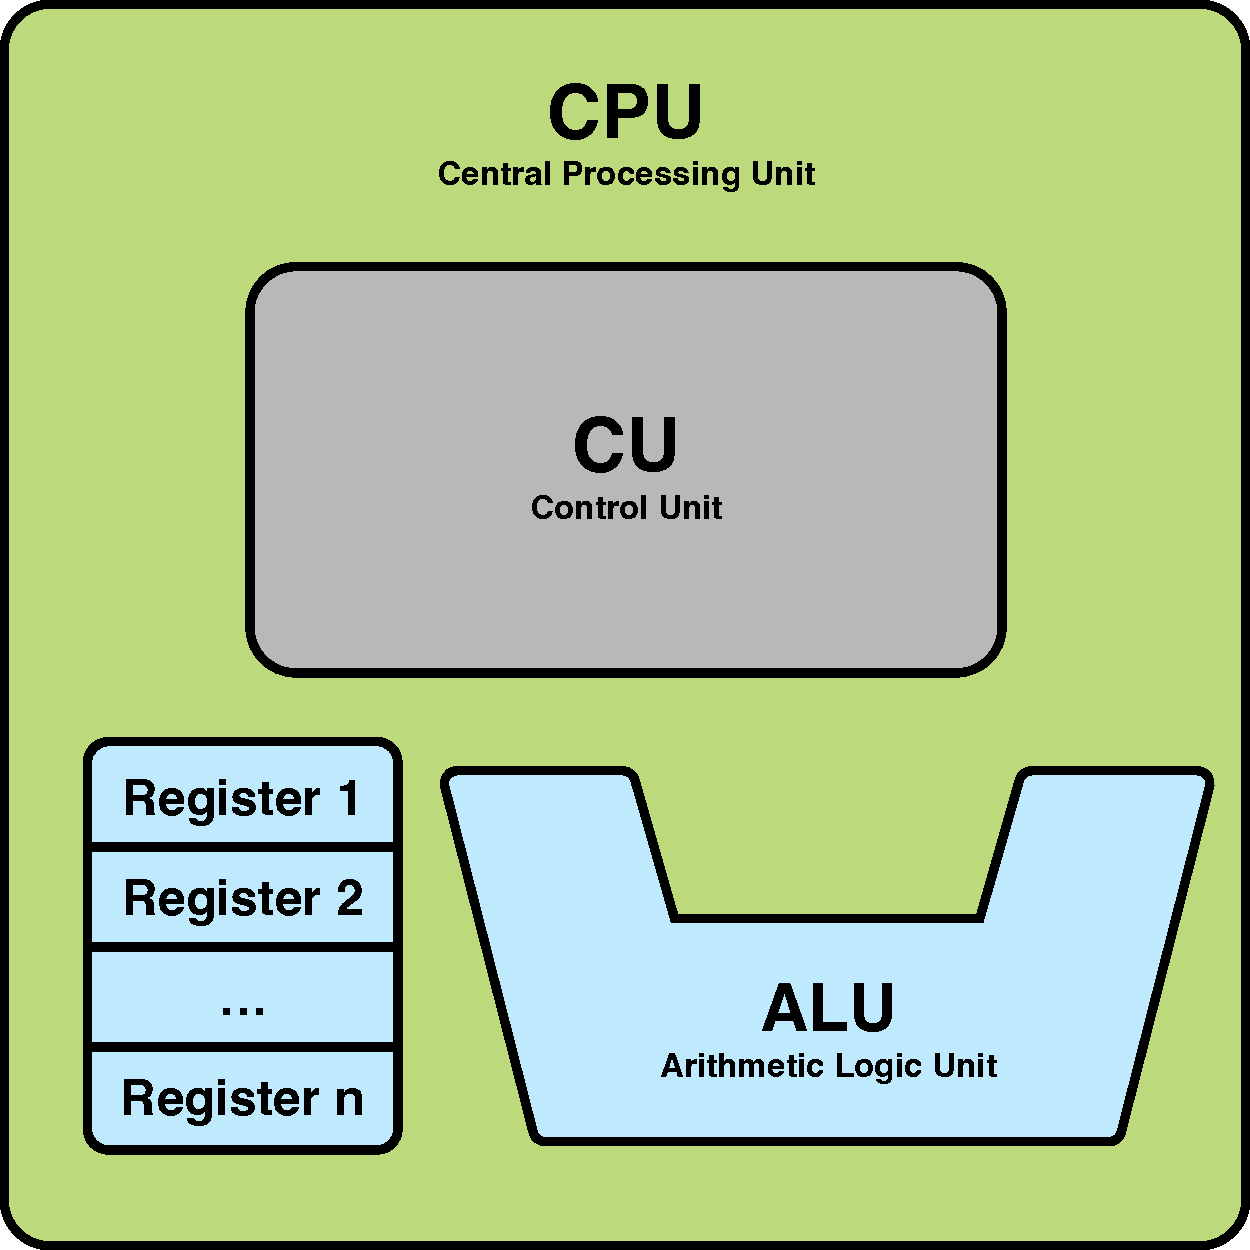
\includegraphics[width=0.58\linewidth]{images/4_cpu/architecture_cpu_simple.pdf}
		\caption{La CPU: CU, ALU e registri}
		\label{fig:cpu_simple}
	\end{figure}
	 
\end{frame}




\subsection[Il ciclo di macchina]{Il ciclo di macchina}

\begin{frame}
	\frametitle{Il ciclo di macchina}
	
	\begin{block}{Il ciclo di macchina}
		 La CPU esegue le istruzioni macchina in maniera ciclica.\\
		 Il cosiddetto \textbf{ciclo di macchina} può essere idealmente suddiviso in 4 parti:
		 
		\begin{columns}			
			\column{0.65\linewidth}
			\begin{enumerate}
			 	\item {\color{CpuGreen}\textbf{fetch}}: prelevamento dalla memoria del codice macchina dell’istruzione da eseguire;
			 	\item {\color{CpuRed}\textbf{decode}}: l'istruzione prelevata viene trasferita in un registro specifico e quindi codificata (tradotta);
			 	\item {\color{CpuBlue}\textbf{fetch operands}}: se necessario si prelevano anche gli operandi necessari all'istruzione;
			 	\item {\color{CpuYellow}\textbf{execute}}: la CPU quindi emette i segnali necessari all'esecuzione dell’istruzione.
			 \end{enumerate}
			
			\column{0.35\linewidth}
			\begin{figure}[!htbp]
				\centering 
				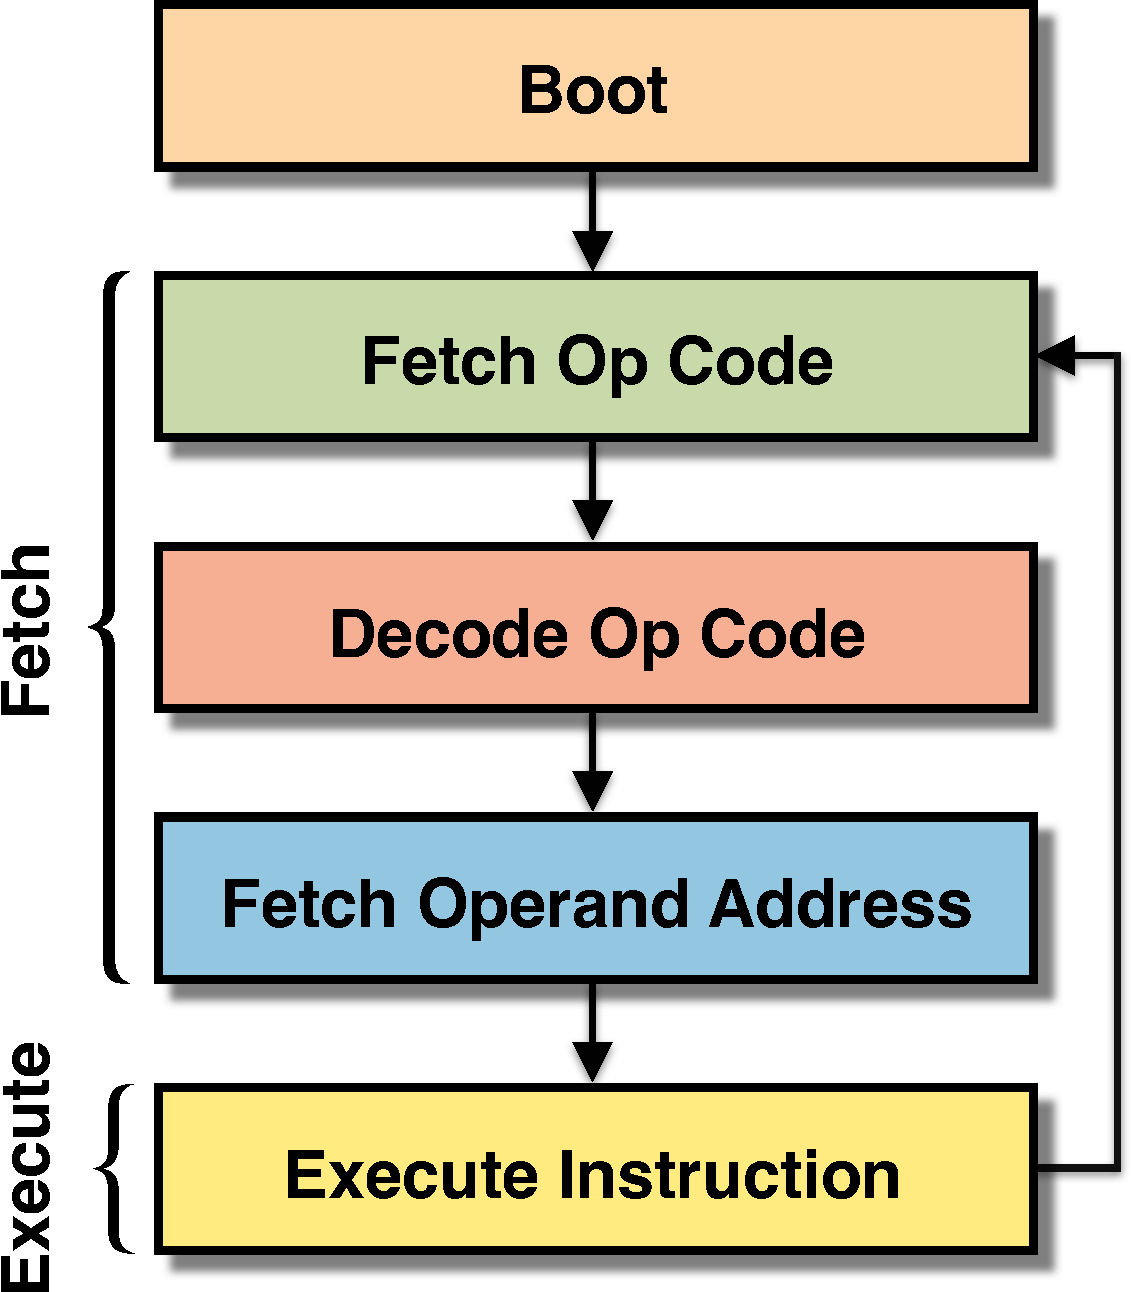
\includegraphics[width=0.95\linewidth]{images/4_cpu/architecture_cpu_cycle.pdf}
%				\caption{}
			\end{figure} 
		\end{columns}
		 
		 
	\end{block}
	
\end{frame}


\begin{frame}
	\frametitle{Il ciclo di macchina: schema della CPU ($\bigstar$)}
	
	\begin{figure}[!htbp] 
		\centering
		%\advance\leftskip-0.25cm
		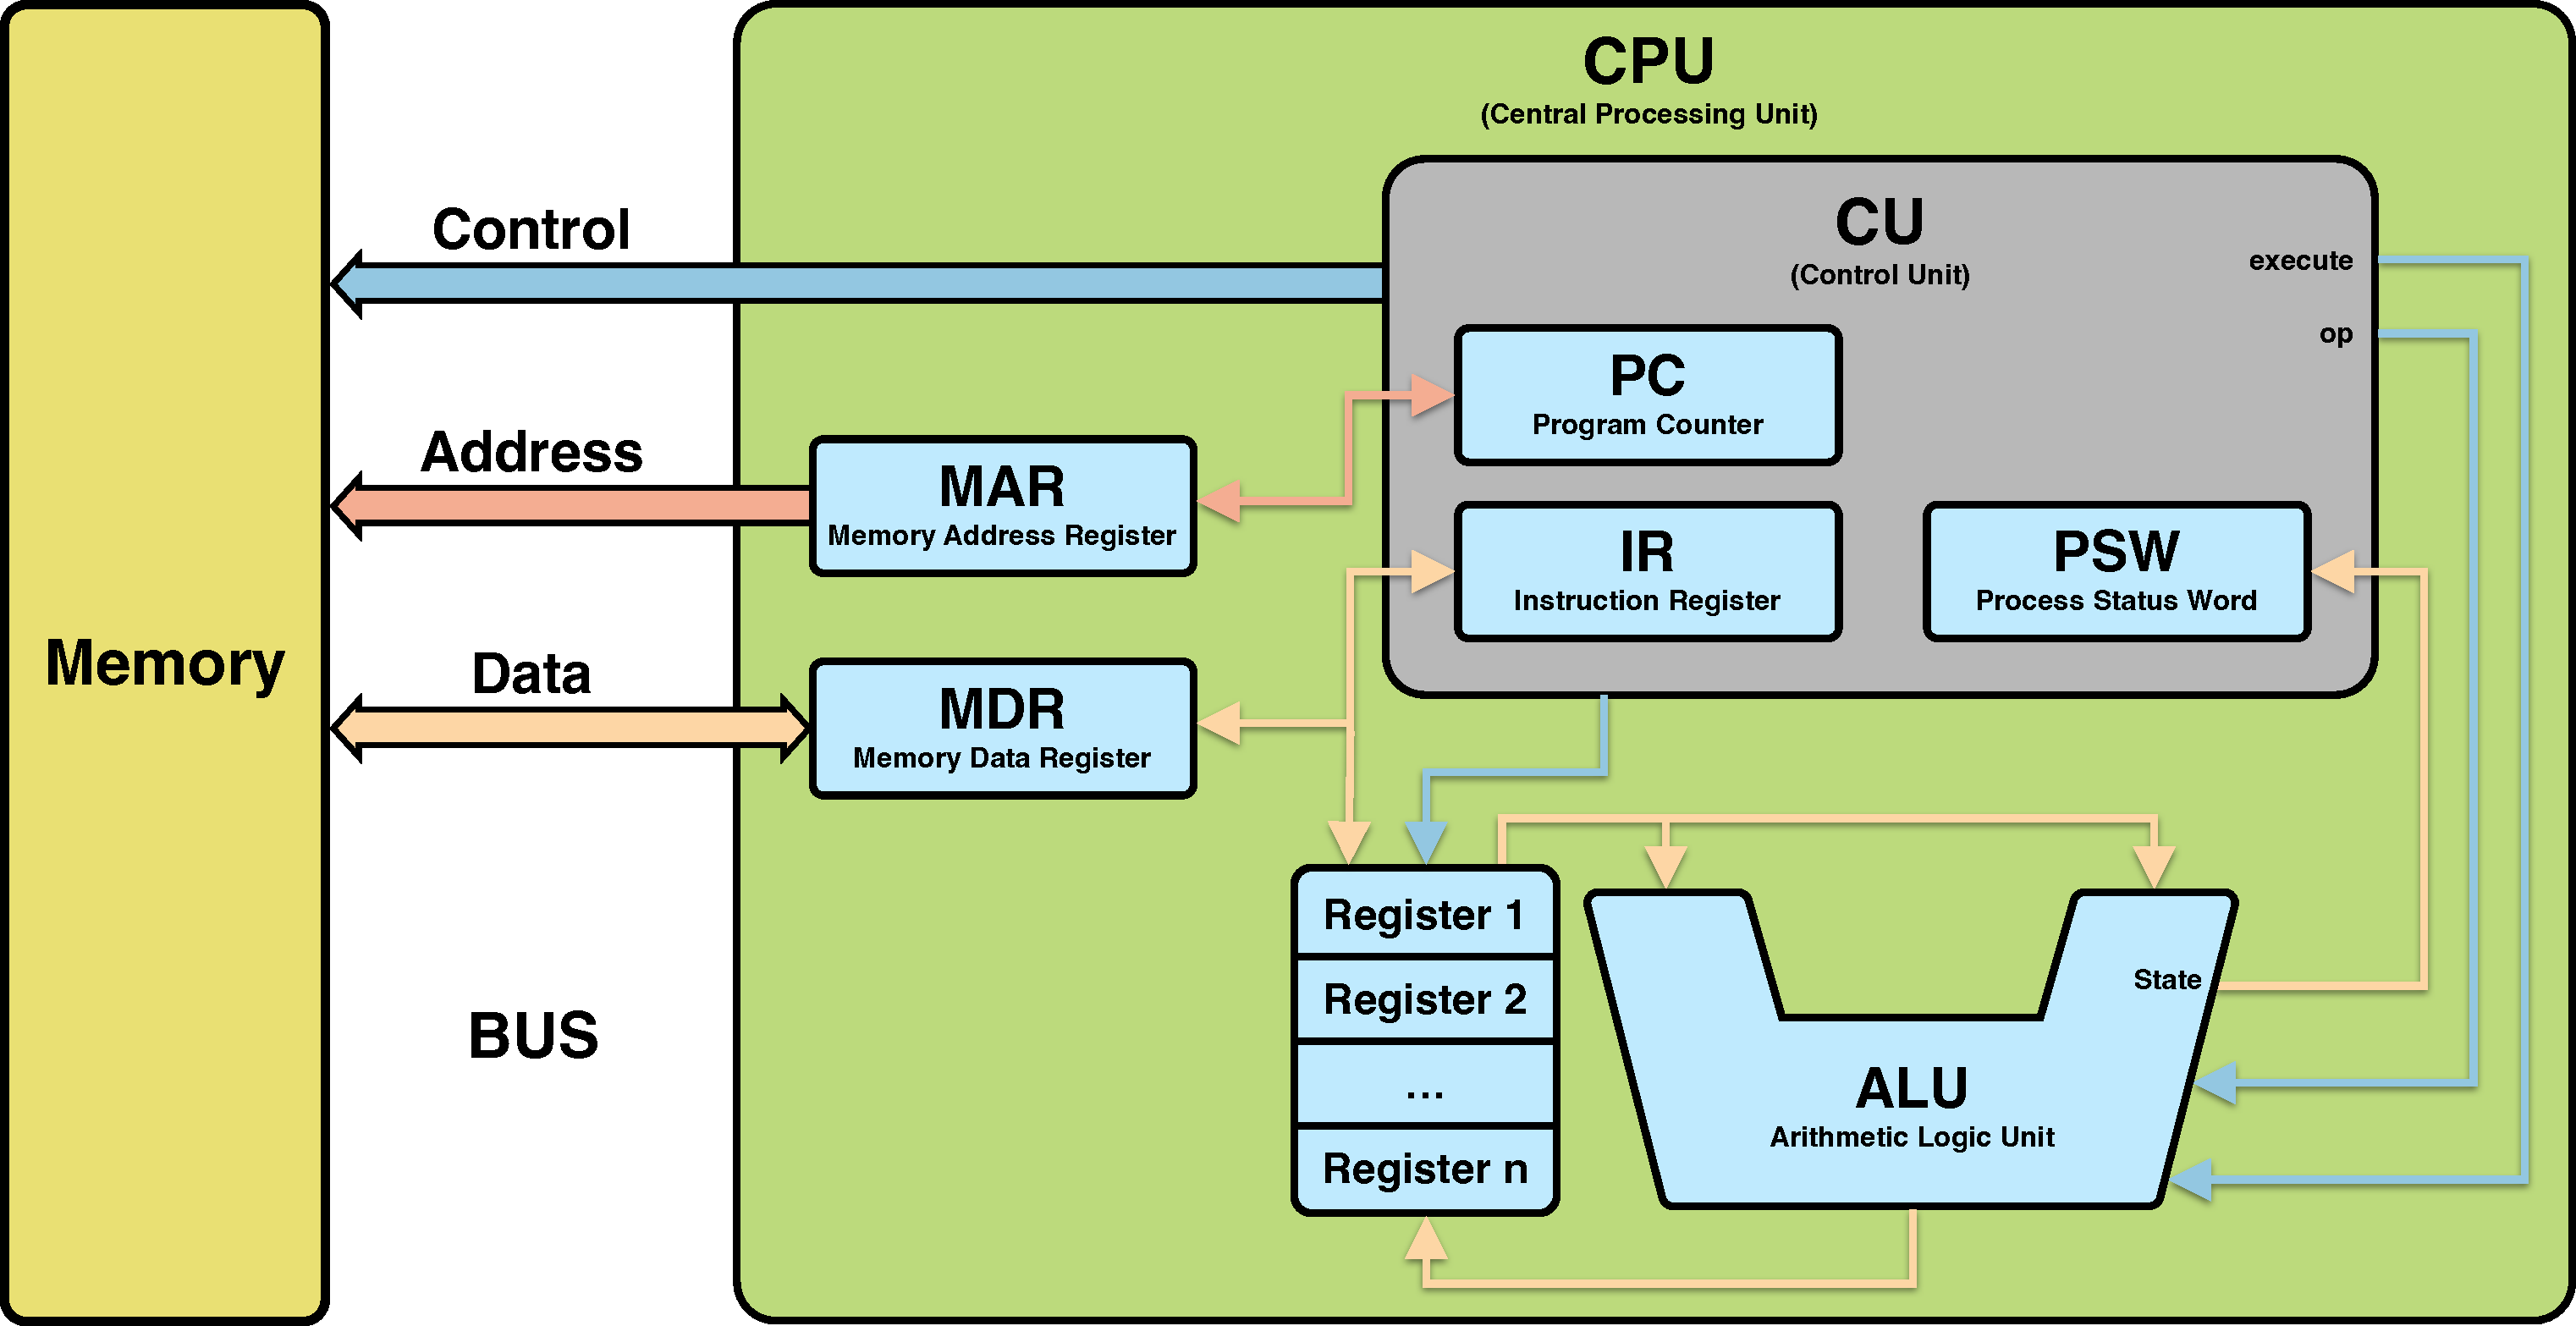
\includegraphics[width=1.0\linewidth]{images/4_cpu/architecture_cpu_complex.pdf}
%		\caption{La CPU: CU, ALU e registri}
		\label{fig:cpu_complex}
	\end{figure}
	 
\end{frame}



\subsubsection[Fetch]{Fetch}
\begin{frame}
	\frametitle{{\color{GradientDescentDiagramGreen}Hierarchical Clustering}}
	\frametitle{Il ciclo di macchina: il {\color{CpuGreen}\textbf{fetch}}}
	
	\begin{block}{Il ciclo di macchina: il fetch}
		\begin{enumerate}
			\item la CPU mette il valore di PC (indirizzo della prossima istruzione da leggere dalla memoria) su MAR e attiva la linea Leggi (Control BUS);
			\item la memoria attraverso il BUS indirizzi accede a MAR e, una volta reperito quanto richiesto, lo scrive su MDR attraverso il BUS dati;
		\end{enumerate}
	\end{block}
	
	\begin{figure}[!htbp] 
		\centering
		%\advance\leftskip-0.25cm
		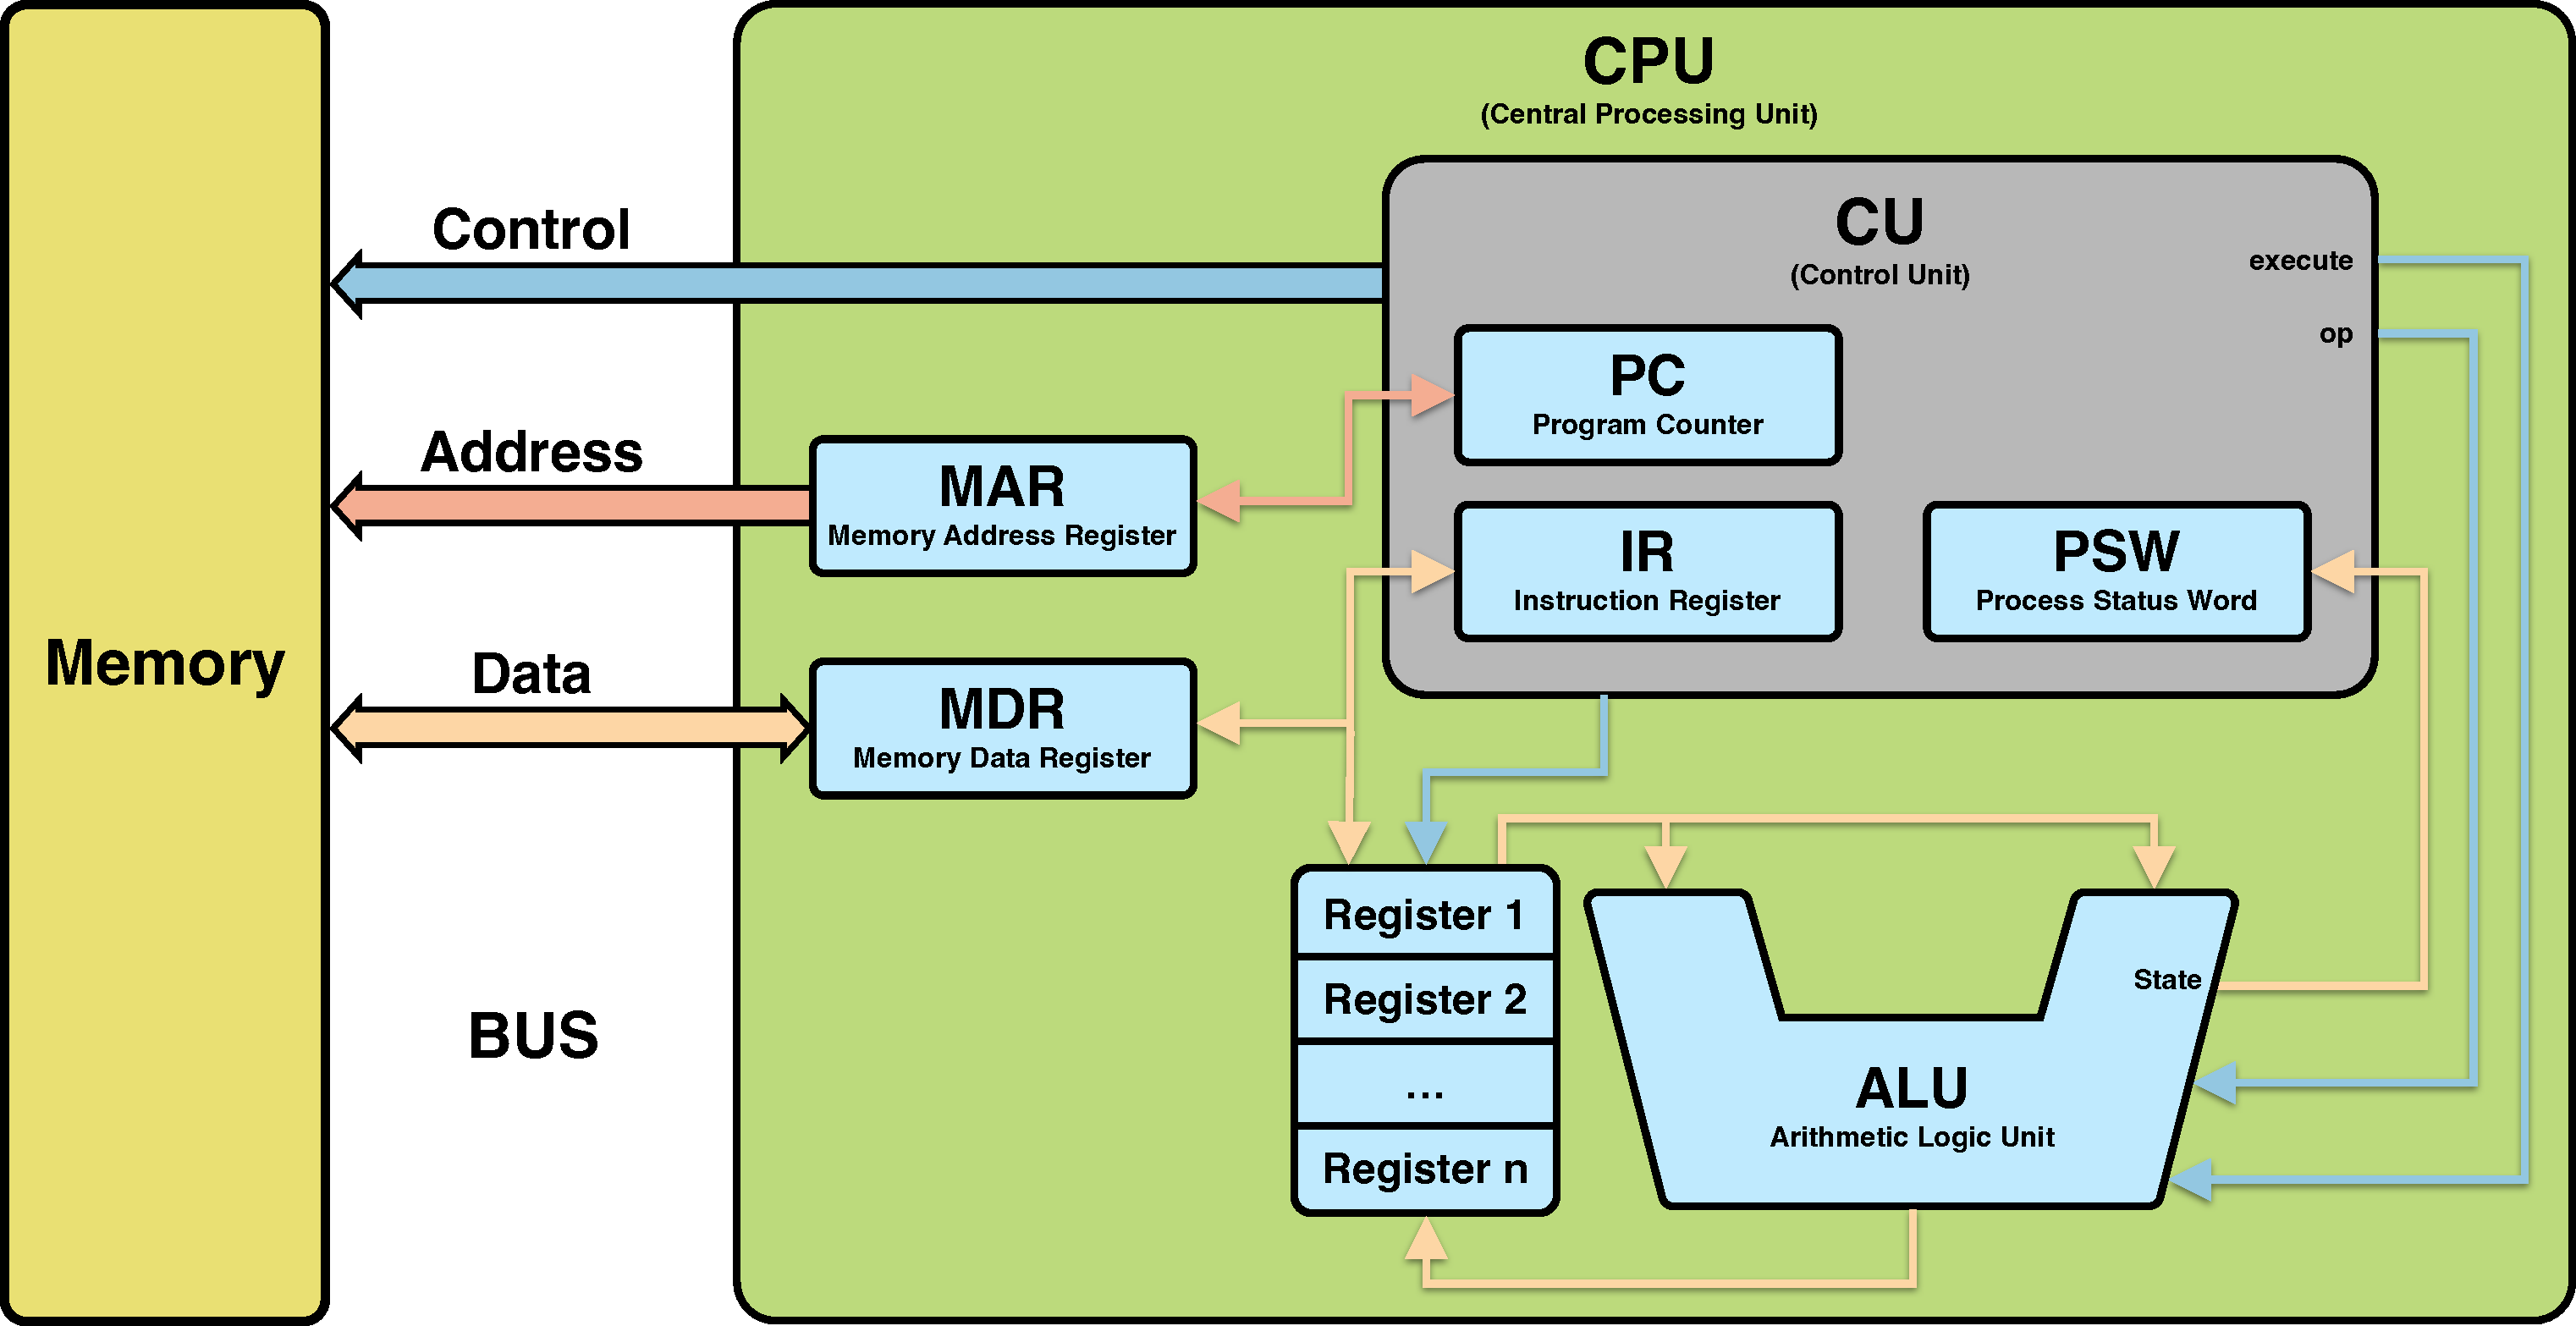
\includegraphics[width=0.7\linewidth]{images/4_cpu/architecture_cpu_complex.pdf}
%		\caption{La CPU: CU, ALU e registri}
		\label{fig:cpu_complex}
	\end{figure}
	
\end{frame}


\subsubsection[Decode]{Decode}
\begin{frame}
	\frametitle{Il ciclo di macchina: il {\color{CpuRed}\textbf{decode}}}
	
	\begin{block}{Il ciclo di macchina: il decode}	
	
		\begin{enumerate}
			\setcounter{enumi}{2}
			\item la CPU copia su IR il valore di MDR e decodifica l'istruzione;
			\item l'istruzione passa in esecuzione sulla ALU;
		\end{enumerate}
	
	\end{block}
	
	\begin{figure}[!htbp] 
		\centering
		%\advance\leftskip-0.25cm
		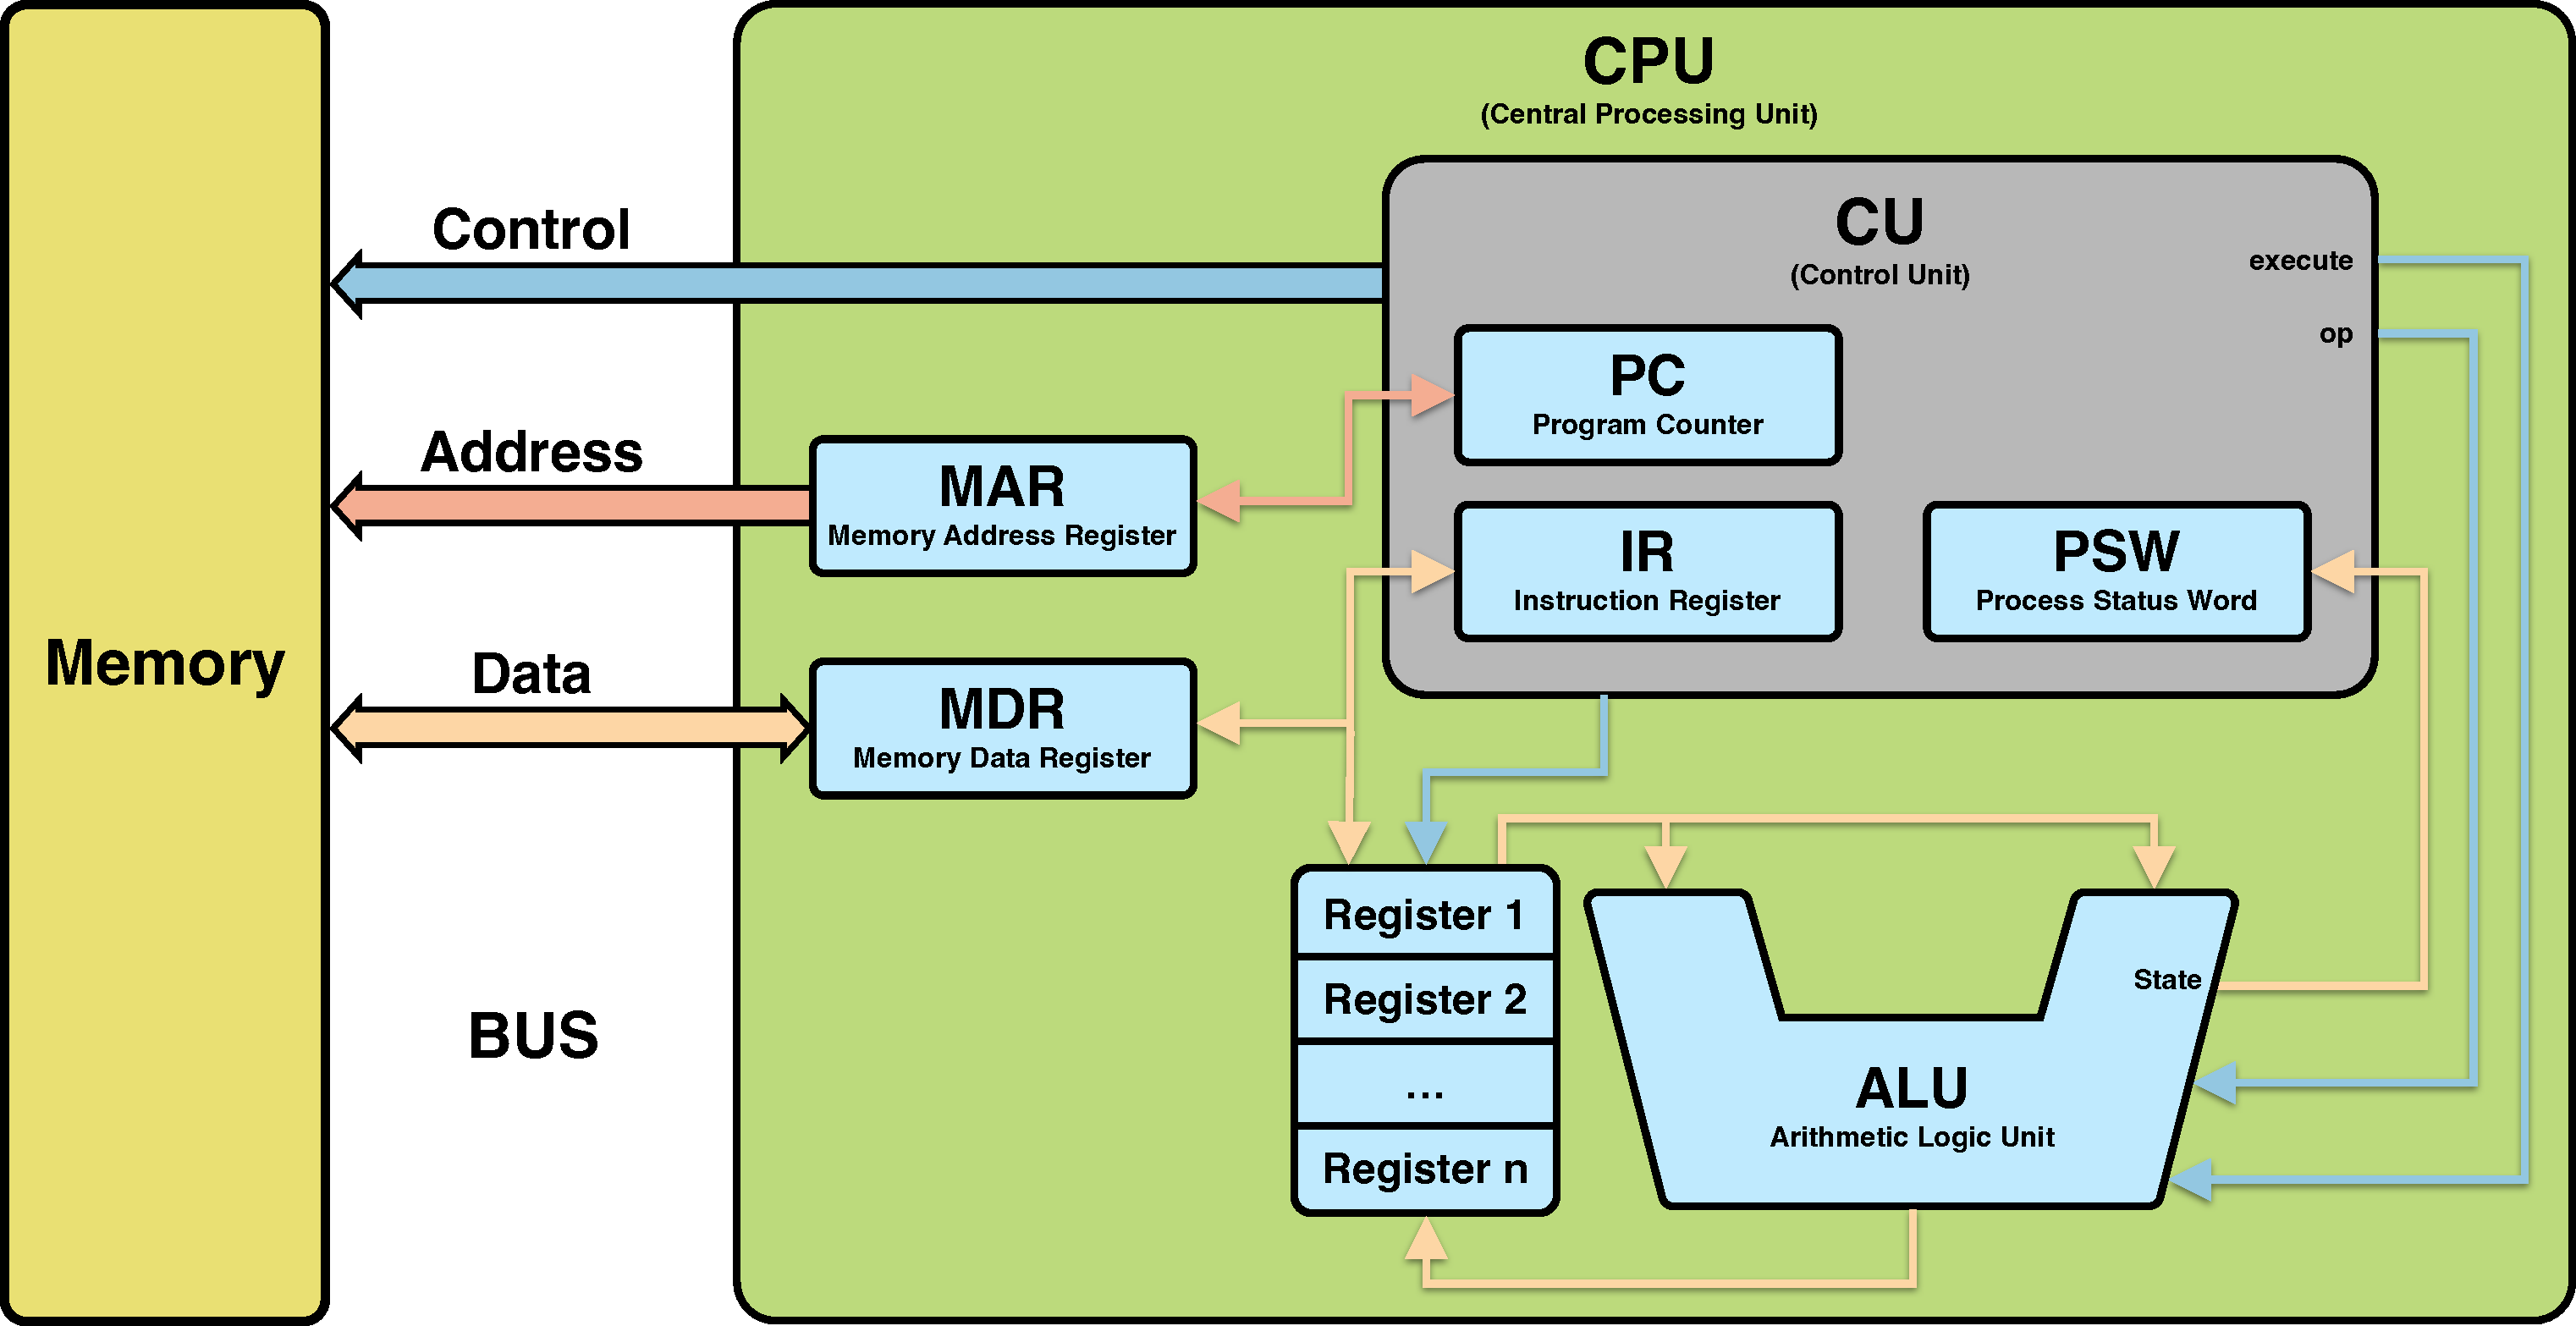
\includegraphics[width=0.7\linewidth]{images/4_cpu/architecture_cpu_complex.pdf}
%		\caption{La CPU: CU, ALU e registri}
		\label{fig:cpu_complex}
	\end{figure}
	
\end{frame}

\subsubsection[Fetch Operands]{Fetch Operands}
\begin{frame}
	\frametitle{Il ciclo di macchina: il {\color{CpuBlue}\textbf{fetch degli operandi}}}
	
	\begin{block}{Il ciclo di macchina: il fetch degli operandi}
		\begin{enumerate}
			\setcounter{enumi}{4}
			\item se l'istruzione prevede la lettura di operandi dalla memoria, questi devono essere caricati sui registri; per ciascun operando da reperire: 
				\begin{enumerate}
					\item la CPU mette l'indirizzo dell'operando su MAR e attiva la linea Leggi;
					\item la memoria attraverso il BUS indirizzi accede a MAR e, una volta reperito quanto richiesto, lo scrive su MDR attraverso il BUS dati;
					\item la CPU copia sul registro destinazione il valore dell'operando che è in MDR;
				\end{enumerate}
			
		\end{enumerate}
	
	\end{block}
	
	\begin{figure}[!htbp] 
		\centering
		%\advance\leftskip-0.25cm
		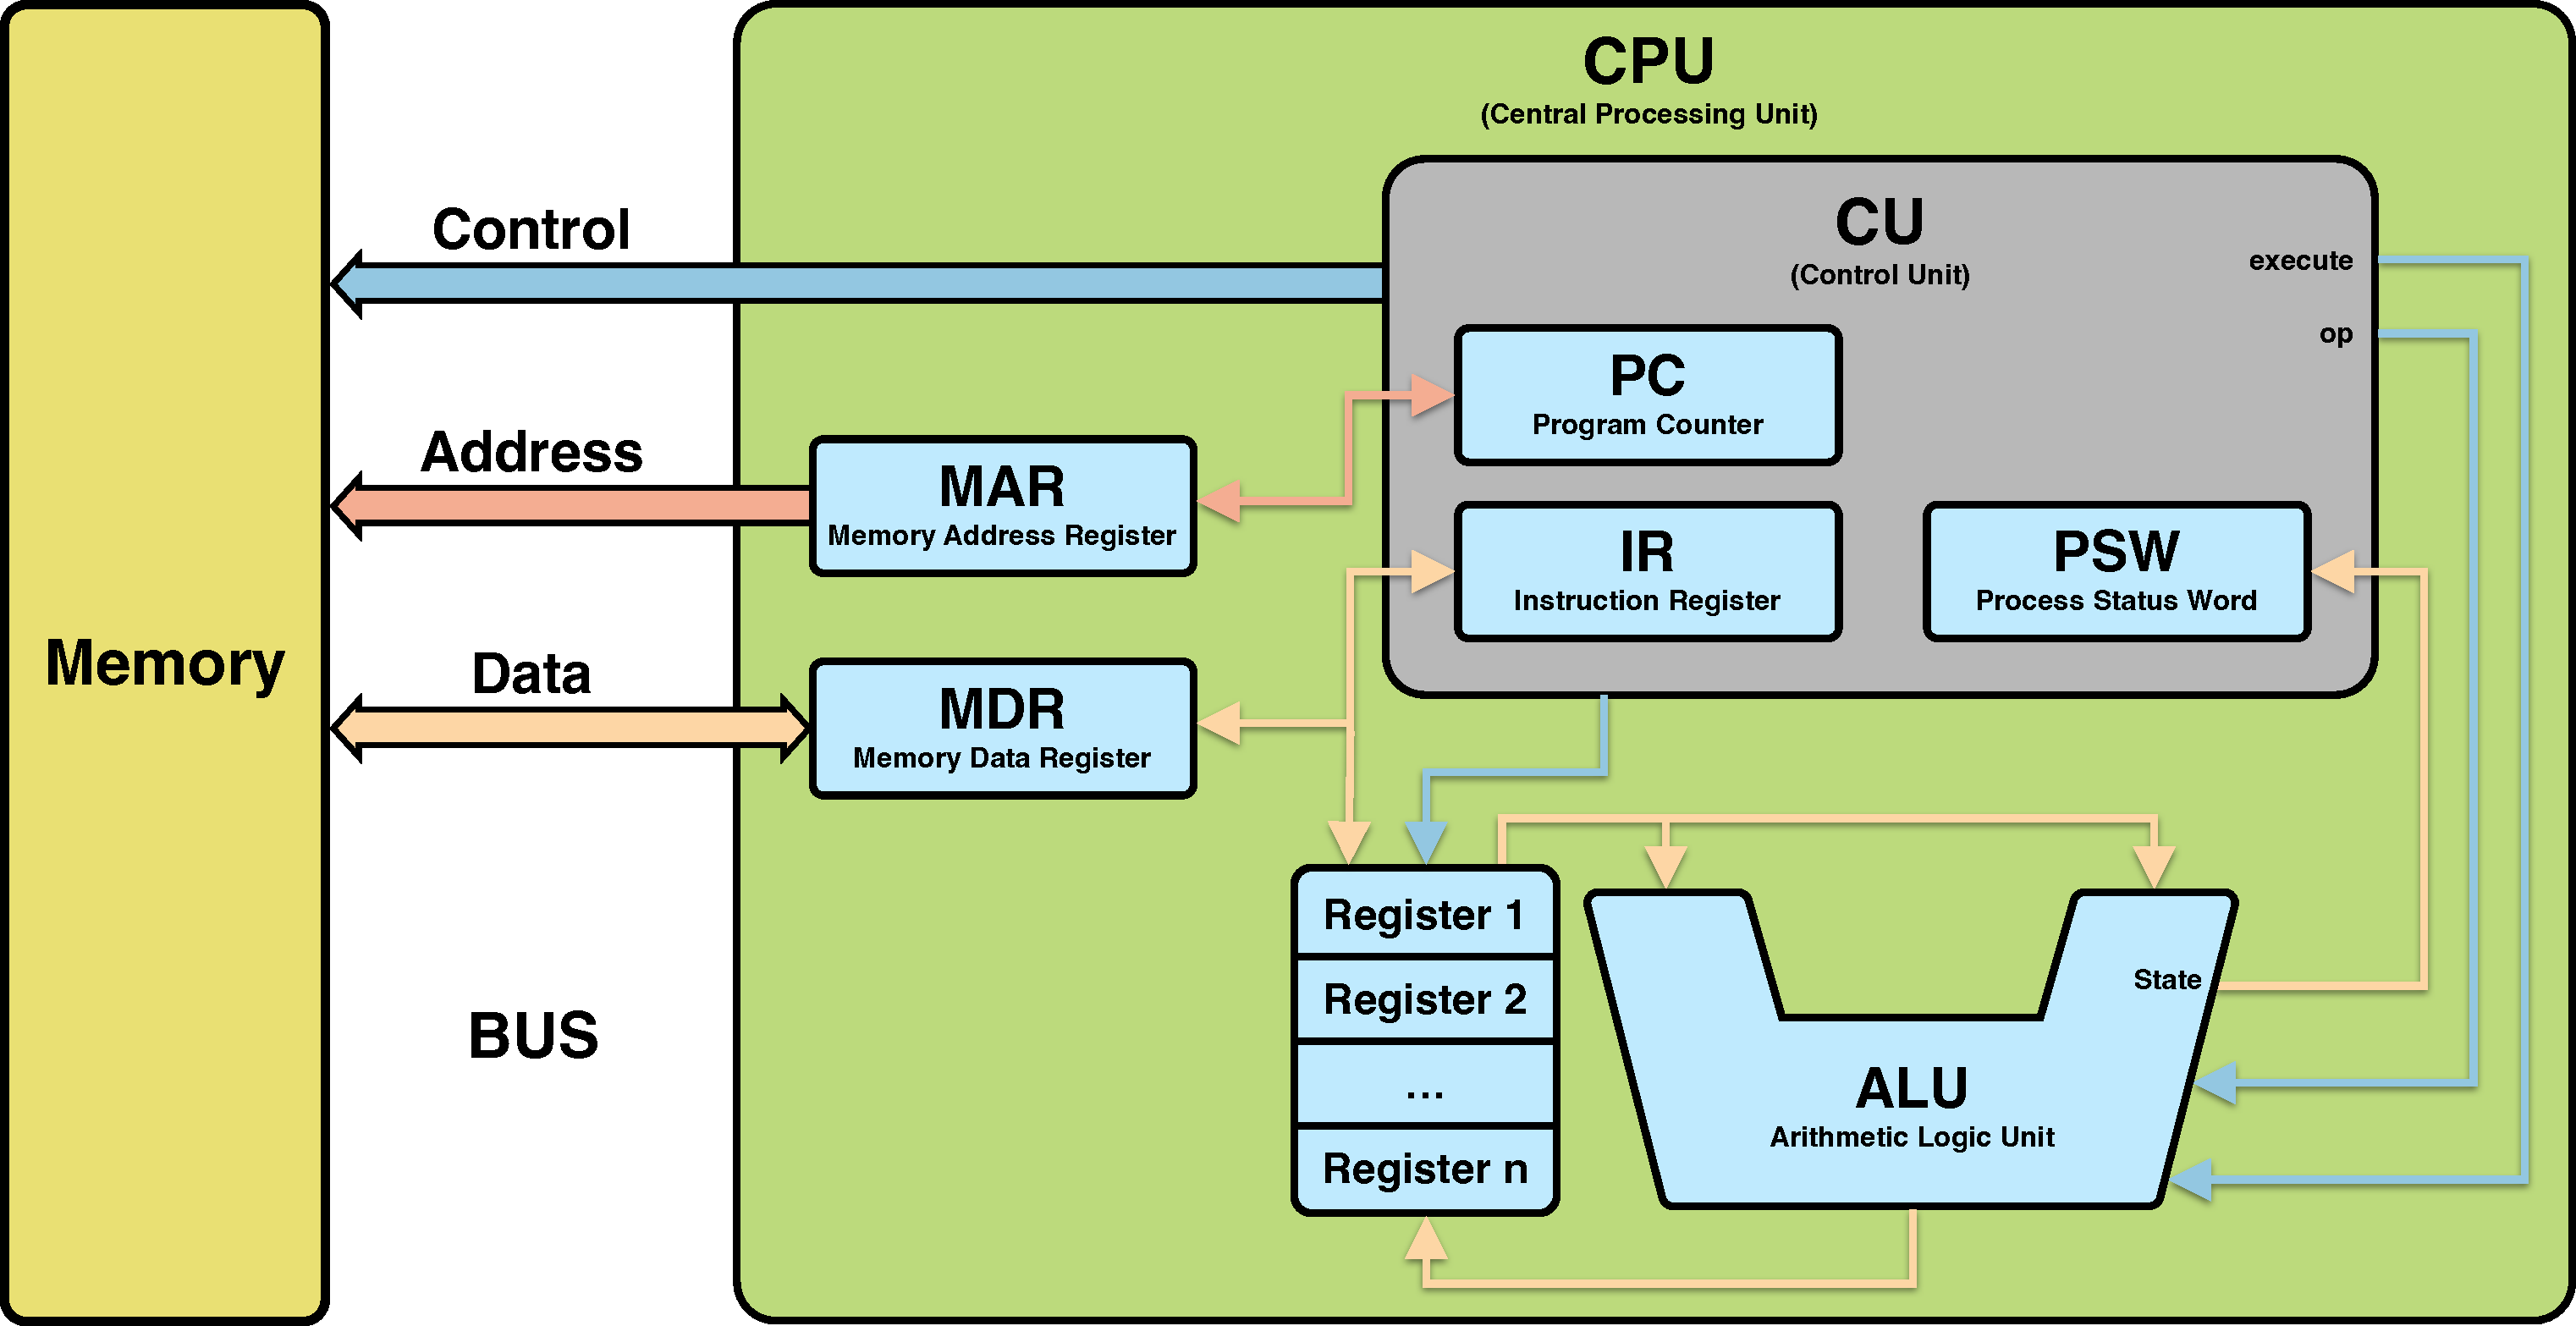
\includegraphics[width=0.51\linewidth]{images/4_cpu/architecture_cpu_complex.pdf}
%		\caption{La CPU: CU, ALU e registri}
		\label{fig:cpu_complex}
	\end{figure}
	
\end{frame}


\subsubsection[Execute]{Execute}
\begin{frame}
	\frametitle{Il ciclo di macchina: l'{\color{CpuYellow}\textbf{execute}}}
	
	\begin{block}{Il ciclo di macchina: l'execute}	
		\begin{enumerate}
			\setcounter{enumi}{5}
			\item terminata l'esecuzione la CPU copia sul registro destinazione il valore prodotto dalla ALU; se è prevista scrittura in memoria del risultato:
				
				\begin{enumerate}
					\item la CPU mette l'indirizzo della cella di destinazione su MAR e il risultato su MDR e attiva la linea Scrivi (Control BUS);
					\item la memoria attraverso il BUS indirizzi accede a MAR, attraverso il BUS dati a MDR e, una volta reperito il valore in MDR, lo scrive sulla propria cella interna indicata da MAR;
				\end{enumerate}
		\end{enumerate}
	
	\end{block}
	
	\begin{figure}[!htbp] 
		\centering
		%\advance\leftskip-0.25cm
		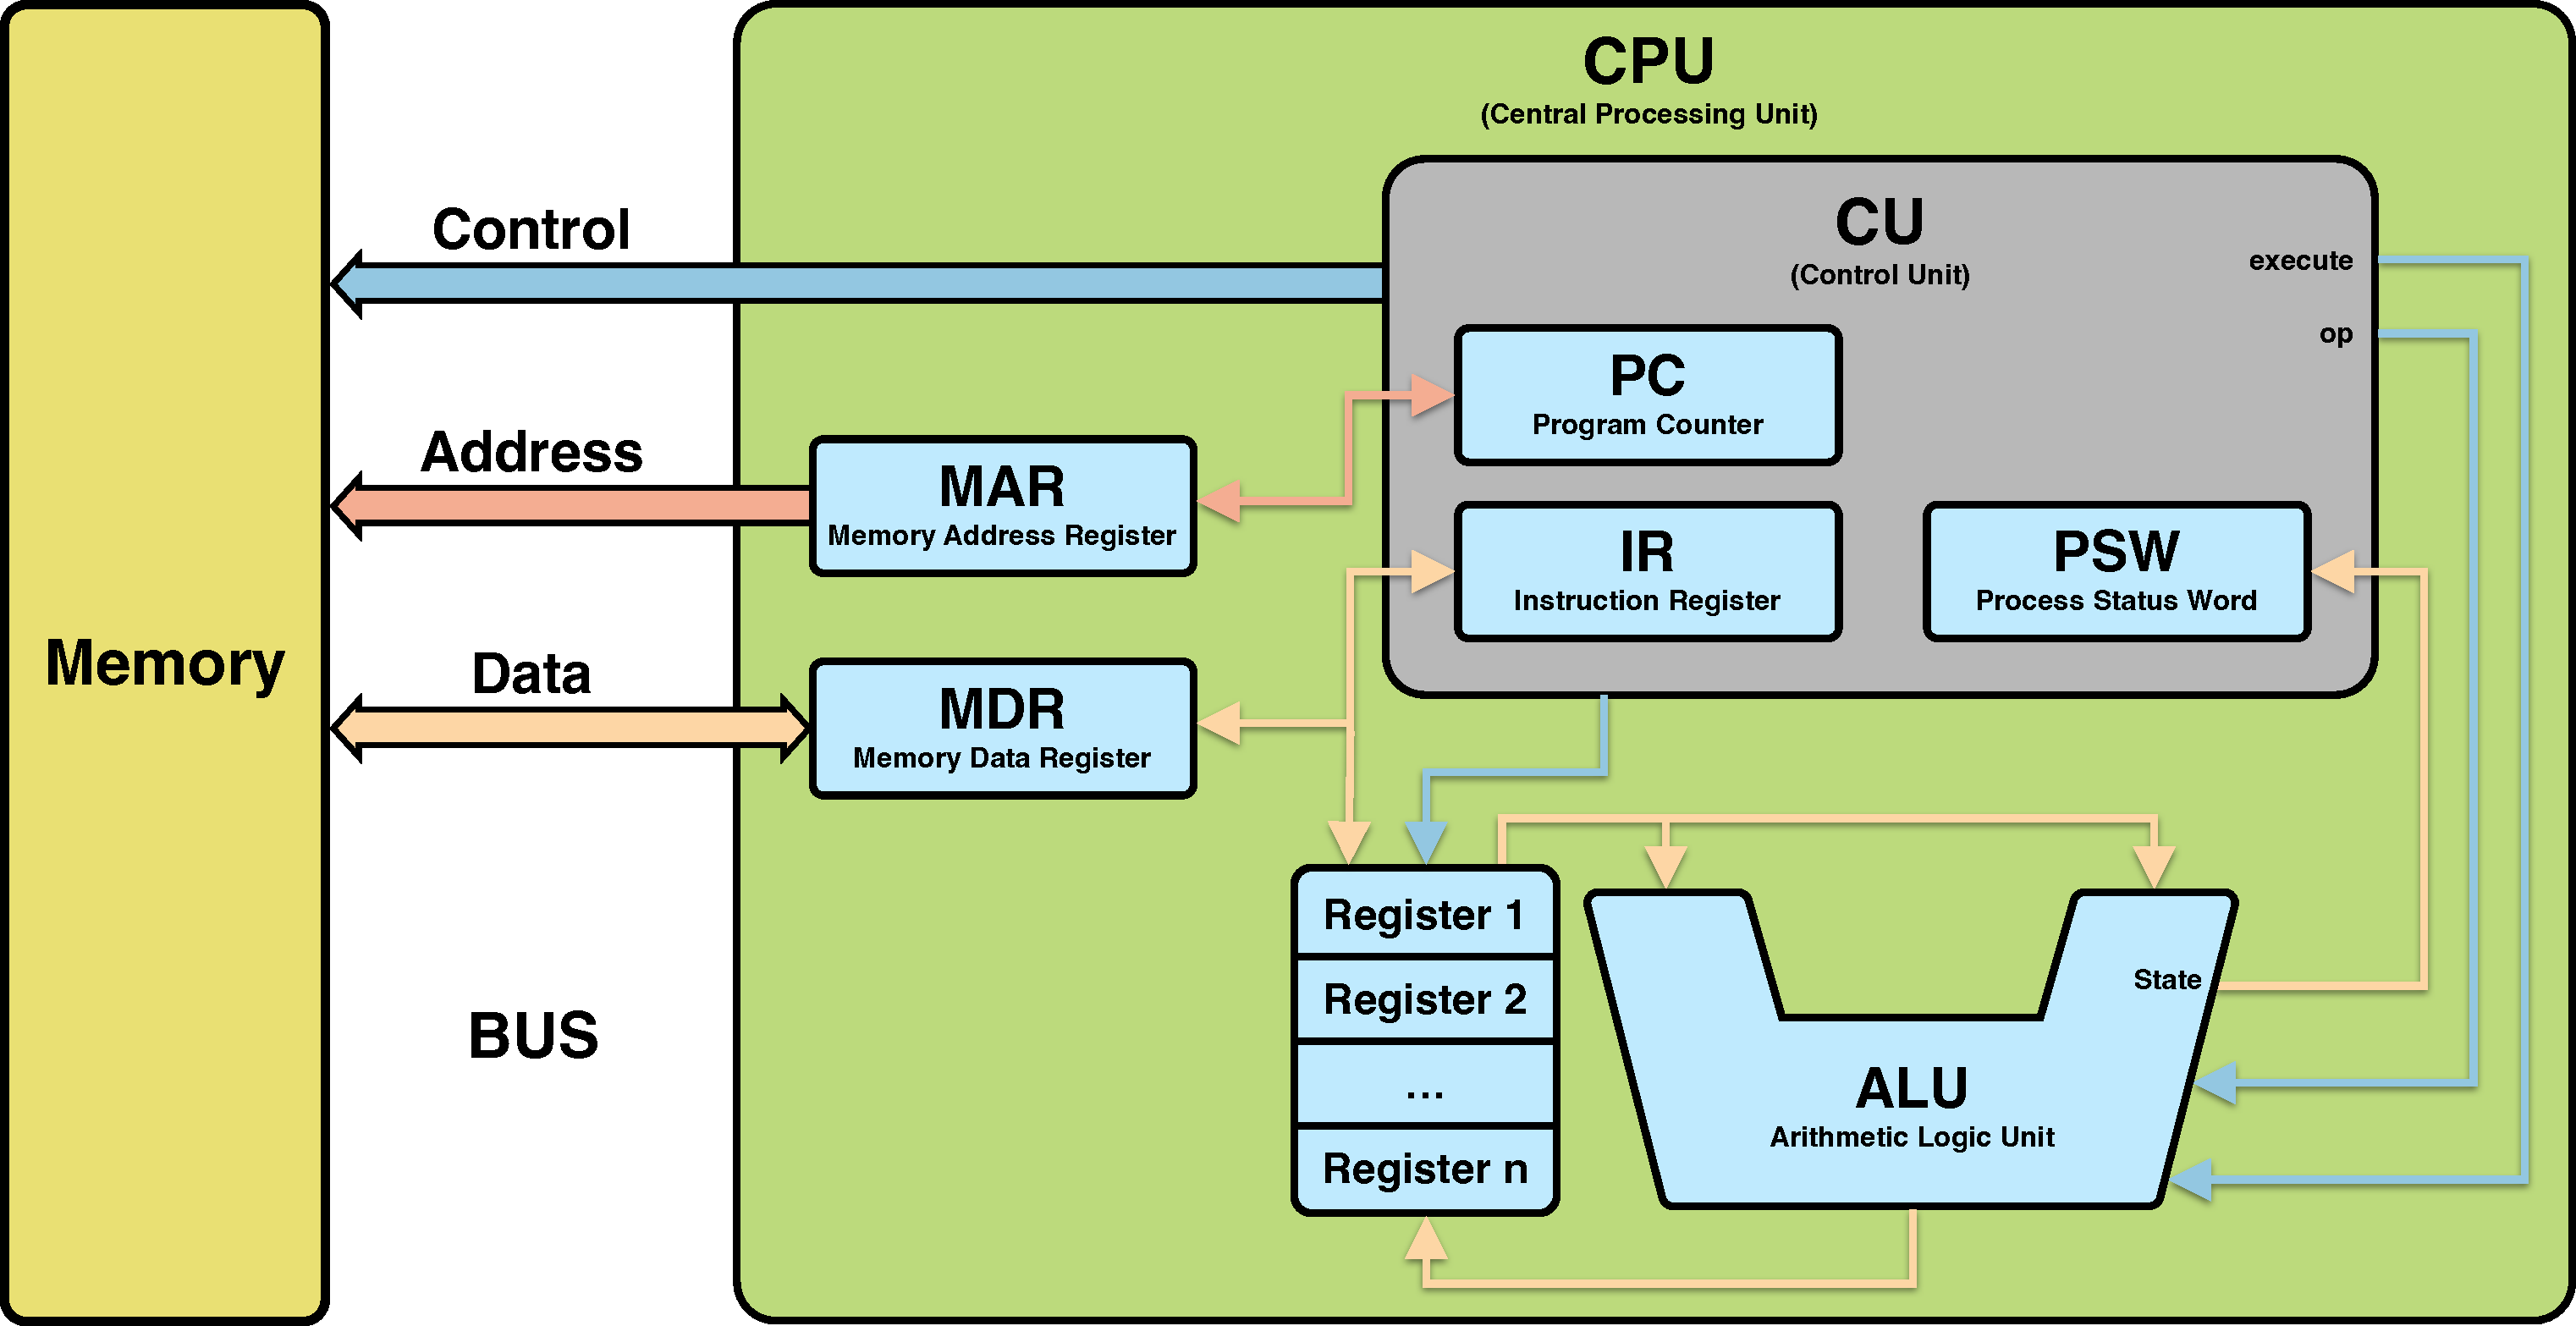
\includegraphics[width=0.51\linewidth]{images/4_cpu/architecture_cpu_complex.pdf}
%		\caption{La CPU: CU, ALU e registri}
		\label{fig:cpu_complex}
	\end{figure}
	
\end{frame}


\begin{frame}
	\frametitle{Il ciclo di macchina: l'{\color{CpuYellow}\textbf{execute}}}
	
	\begin{block}{Il ciclo di macchina: l'execute}	
		\begin{enumerate}
			\setcounter{enumi}{6}
			\item Si ritorna al punto 1 dopo aver aggiornato il valore di PC (prossima istruzione da eseguire).
		\end{enumerate}
	
	\end{block}
	
	\begin{figure}[!htbp] 
		\centering
		%\advance\leftskip-0.25cm
		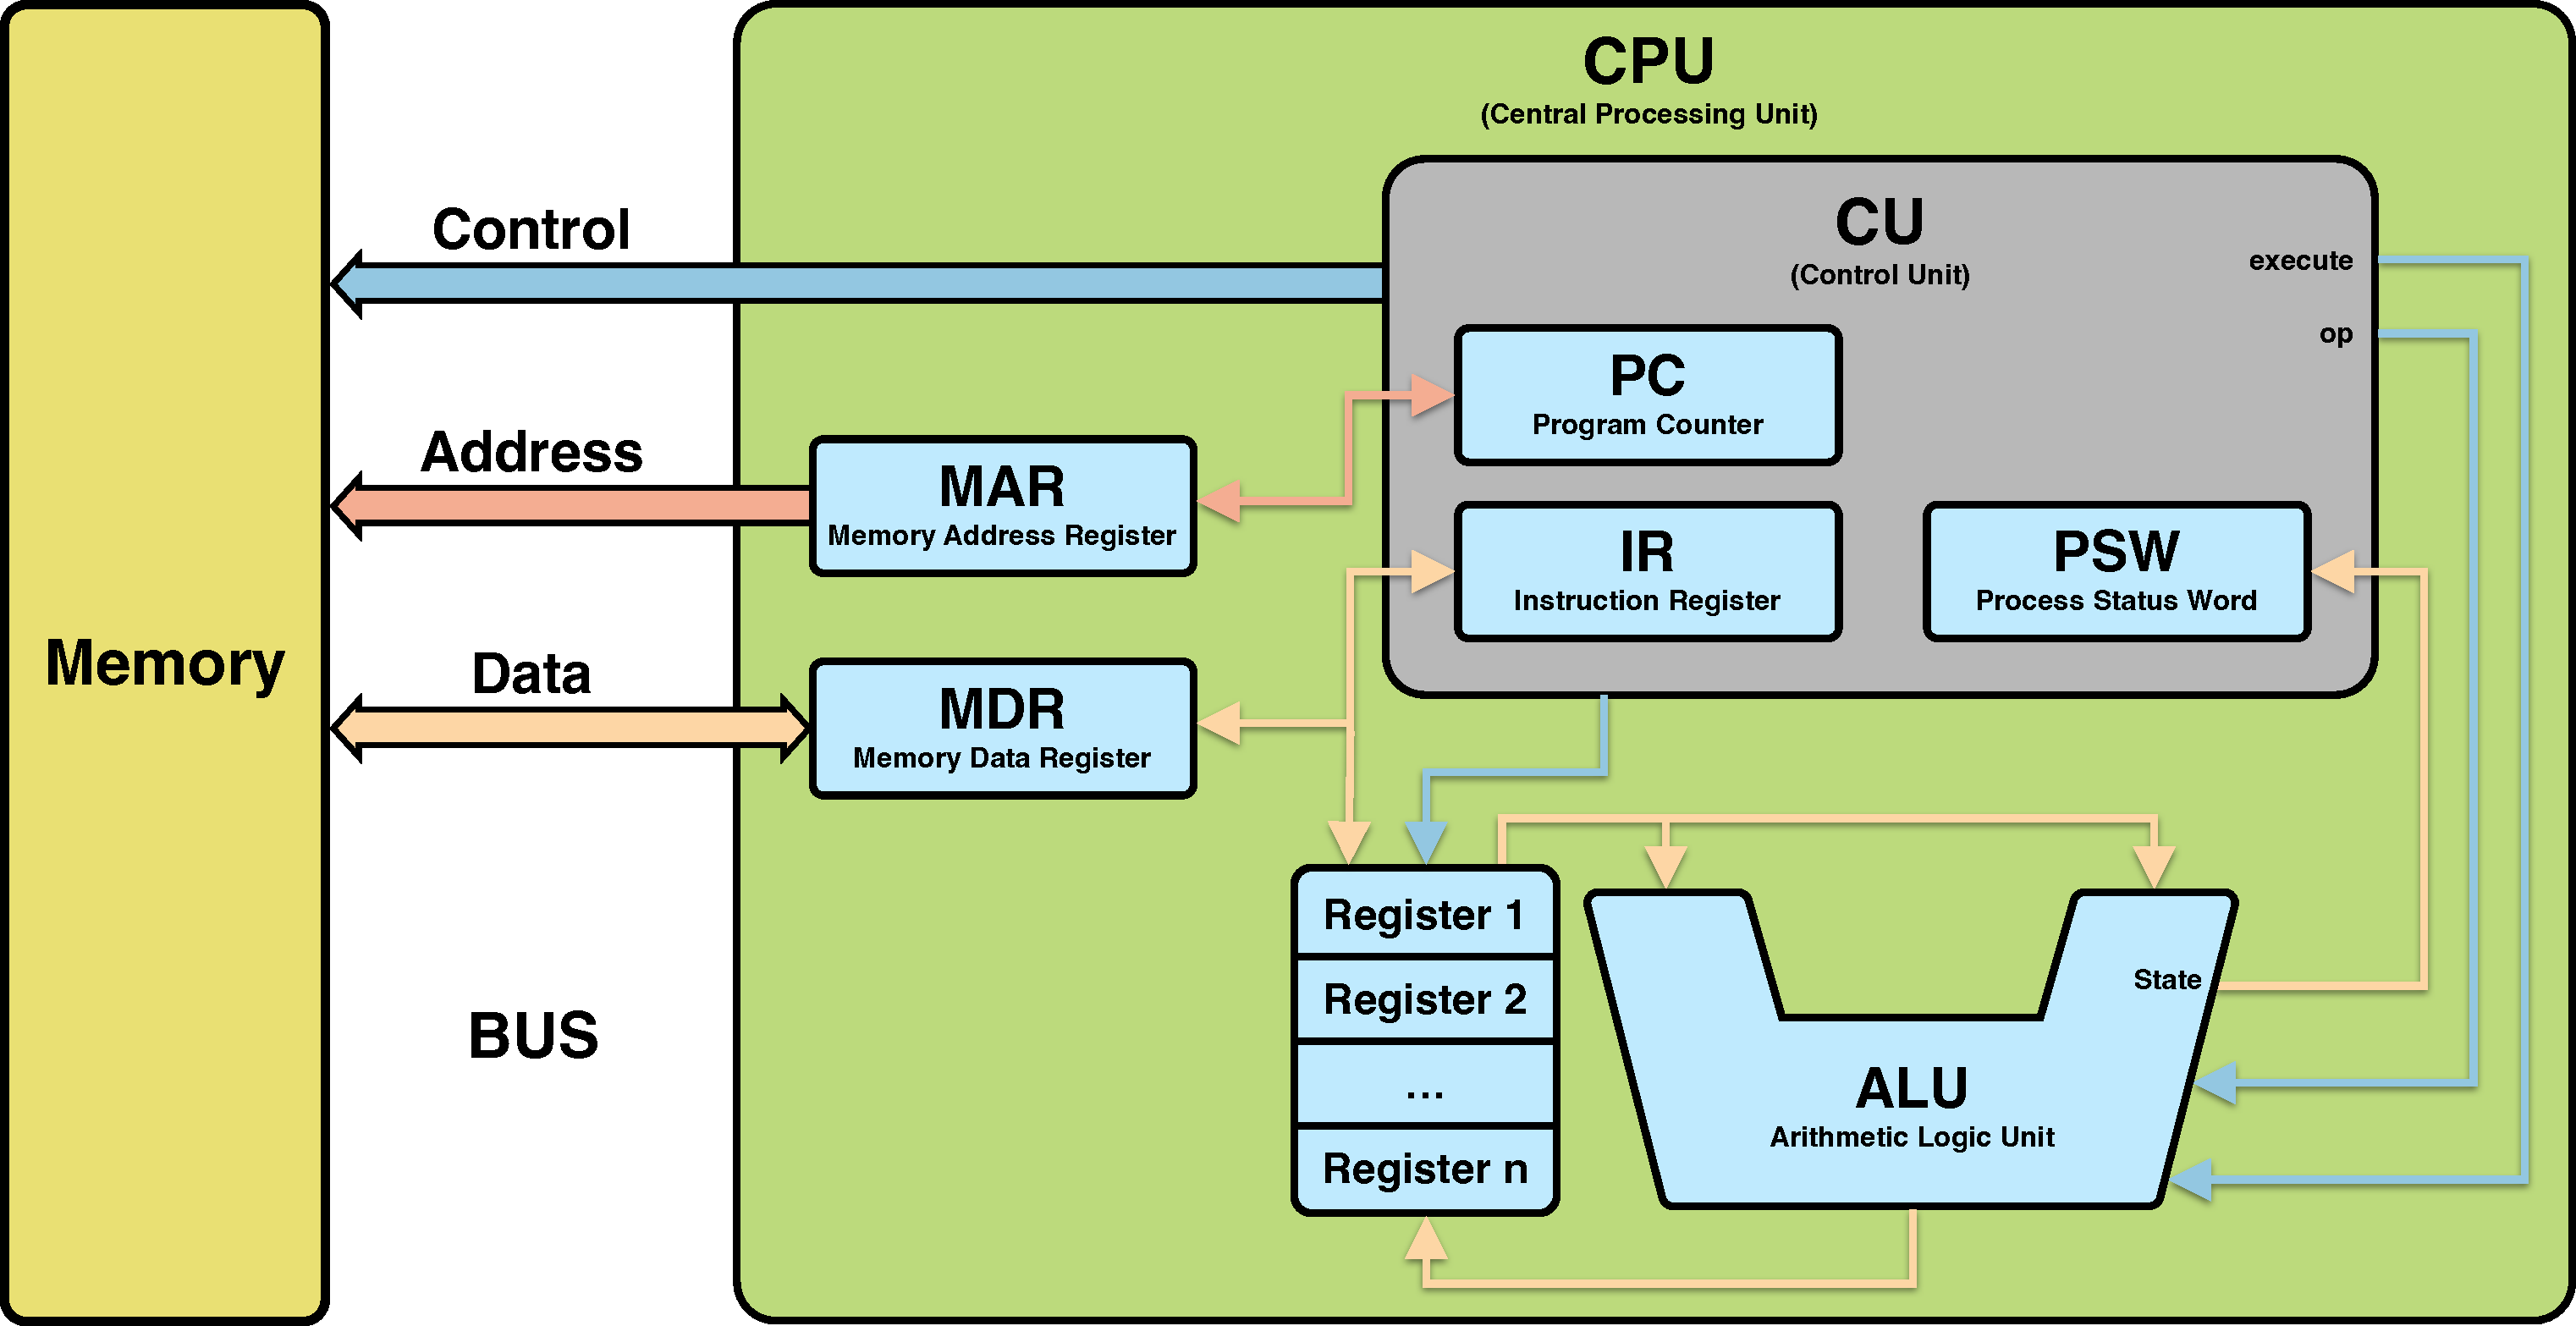
\includegraphics[width=0.7\linewidth]{images/4_cpu/architecture_cpu_complex.pdf}
%		\caption{La CPU: CU, ALU e registri}
		\label{fig:cpu_complex}
	\end{figure}
	
\end{frame}

